<<<<<<< HEAD:Exam-2018/Rapport/latex/UserGuide.tex
\documentclass[../master.tex]{subfiles}

=======
\documentclass[../master.tex]{subfile}
>>>>>>> 7b917b593add2c3820e2e9406fd9ec8a3b7c9cf5:Rapport/latex/UserGuide.tex
\begin{document}

\section{User Guide}
To run SpaceTaxi, clone our project (see URL on the front page), open SU18-Exercises/SpaceTaxi-1/SpaceTaxi-1.sln in your preferable IDE, and run the SpaceTaxi-1.sln solution.\\

When starting the game, you will be introduced to the main menu screen. In the main menu you can choose to start a new game or to quit the game. The controls in the menu, where you can select between each interaction choice, you should use the following keys:\\
\begin{wrapfigure}{l}{0.03\textwidth}
	\vspace{-6.9mm}
	\begin{centering}
		
\includegraphics[width=0.04\textwidth]{./Pictures/Pil_op.png}
	\end{centering}
	\vspace{-6mm}
\end{wrapfigure}
Go one choice up.\\

\begin{wrapfigure}{l}{0.03\textwidth}
	\vspace{-6.9mm}
	\begin{centering}
		
\includegraphics[width=0.04\textwidth]{./Pictures/Pil_ned.png}
	\end{centering}
	\vspace{-6mm}
\end{wrapfigure}
Go one choice down.\\

\begin{wrapfigure}{l}{0.03\textwidth}
	\vspace{-6.9mm}
	\begin{centering}
		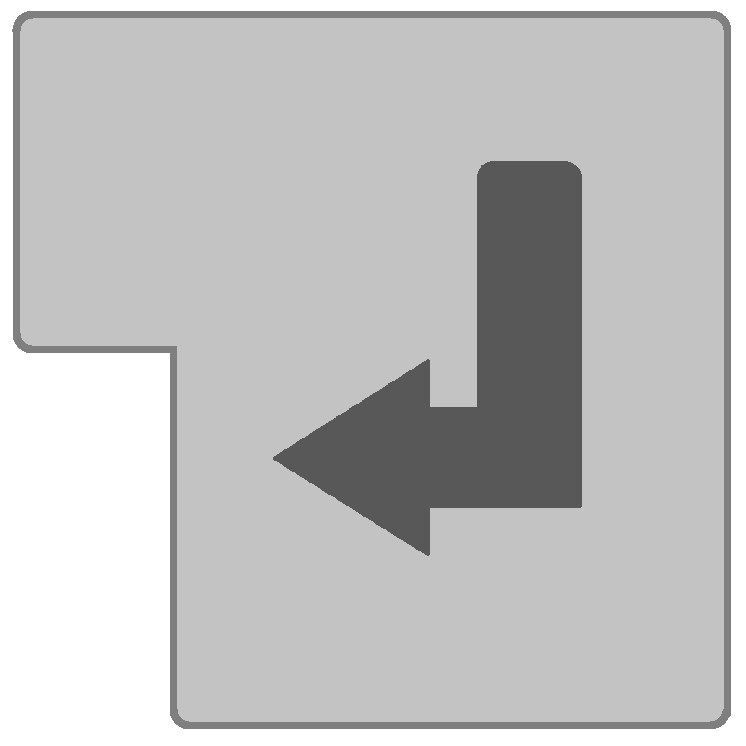
\includegraphics[width=0.04\textwidth]{./Pictures/Enter.png}
	\end{centering}
	\vspace{-6mm}
\end{wrapfigure}
To select your chosen menu button, press enter.\\

If you choose ``New Game``, it will start up the game, while if you choose ``Quit``, it will Quit the game. So if you choose ``New Game`` the game will start, where you will see your ship in the top right corner of the screen placed beside the sugar cane on the left side. The game will begin when you press one of the keys. Then the ship will begin to fall and will keep falling until you hit an obstacle and explode or when you hit the up key that gradually will stop the ship from falling and push the ship upwards. You can also move the ship to left and right. However, be careful as your ship is being affected by physics (gravity and acceleration). If you are going too fast or moving your ship uncontrollable, you may hit an obstacle on the way and the cause will kill both you and your customer. To move your ship, you will use the following keys:\\
\begin{wrapfigure}{l}{0.03\textwidth}
	\vspace{-6.9mm}
	\begin{centering}
		
\includegraphics[width=0.04\textwidth]{./Pictures/Pil_op.png}
	\end{centering}
	\vspace{-6mm}
\end{wrapfigure}
Will accelerate the ship upwards.\\

\begin{wrapfigure}{l}{0.03\textwidth}
	\vspace{-6.9mm}
	\begin{centering}
		
\includegraphics[width=0.04\textwidth]{./Pictures/Pil_venstre.png}
	\end{centering}
	\vspace{-6mm}
\end{wrapfigure}
Will accelerate the ship to the left.\\

\begin{wrapfigure}{l}{0.03\textwidth}
	\vspace{-6.9mm}
	\begin{centering}
		
\includegraphics[width=0.04\textwidth]{./Pictures/Pil_right.png}
	\end{centering}
	\vspace{-6mm}
\end{wrapfigure}
Will accelerate the ship to the right.\\

If you want a break from the game, you can do that by pausing the game. If you want to quit the game, you can do it inside the pause menu, as well. As well as starting a new game. To do the following things you need to use:\\
\begin{wrapfigure}{l}{0.03\textwidth}
	\vspace{-6.6mm}
	\begin{centering}
		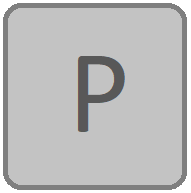
\includegraphics[width=0.04\textwidth]{./Pictures/Pause.png}
	\end{centering}
	\vspace{-6mm}
\end{wrapfigure}
Hit the P-key on the keyboard to pause the game.\\

\begin{wrapfigure}{l}{0.03\textwidth}
	\vspace{-6.9mm}
	\begin{centering}
		
\includegraphics[width=0.04\textwidth]{./Pictures/Quit.png}
	\end{centering}
	\vspace{-6mm}
\end{wrapfigure}
After hitting P-key, press Q to quit the game.\\

\begin{wrapfigure}{l}{0.03\textwidth}
	\vspace{-6.9mm}
	\begin{centering}
		
\includegraphics[width=0.04\textwidth]{./Pictures/New_Game.png}
	\end{centering}
	\vspace{-6mm}
\end{wrapfigure}
After hitting P-key, press N to start a new game.\\

\newpage

\subsection{Game guide}
When running the game you will start in the Main Menu, where you can choose ``New Game'', that will start the game and ``Quit'', that will quit the game. The options which are green, is there you currently is. So if you move one option down, the Quit option will then be green.
\begin{figure}[h]
	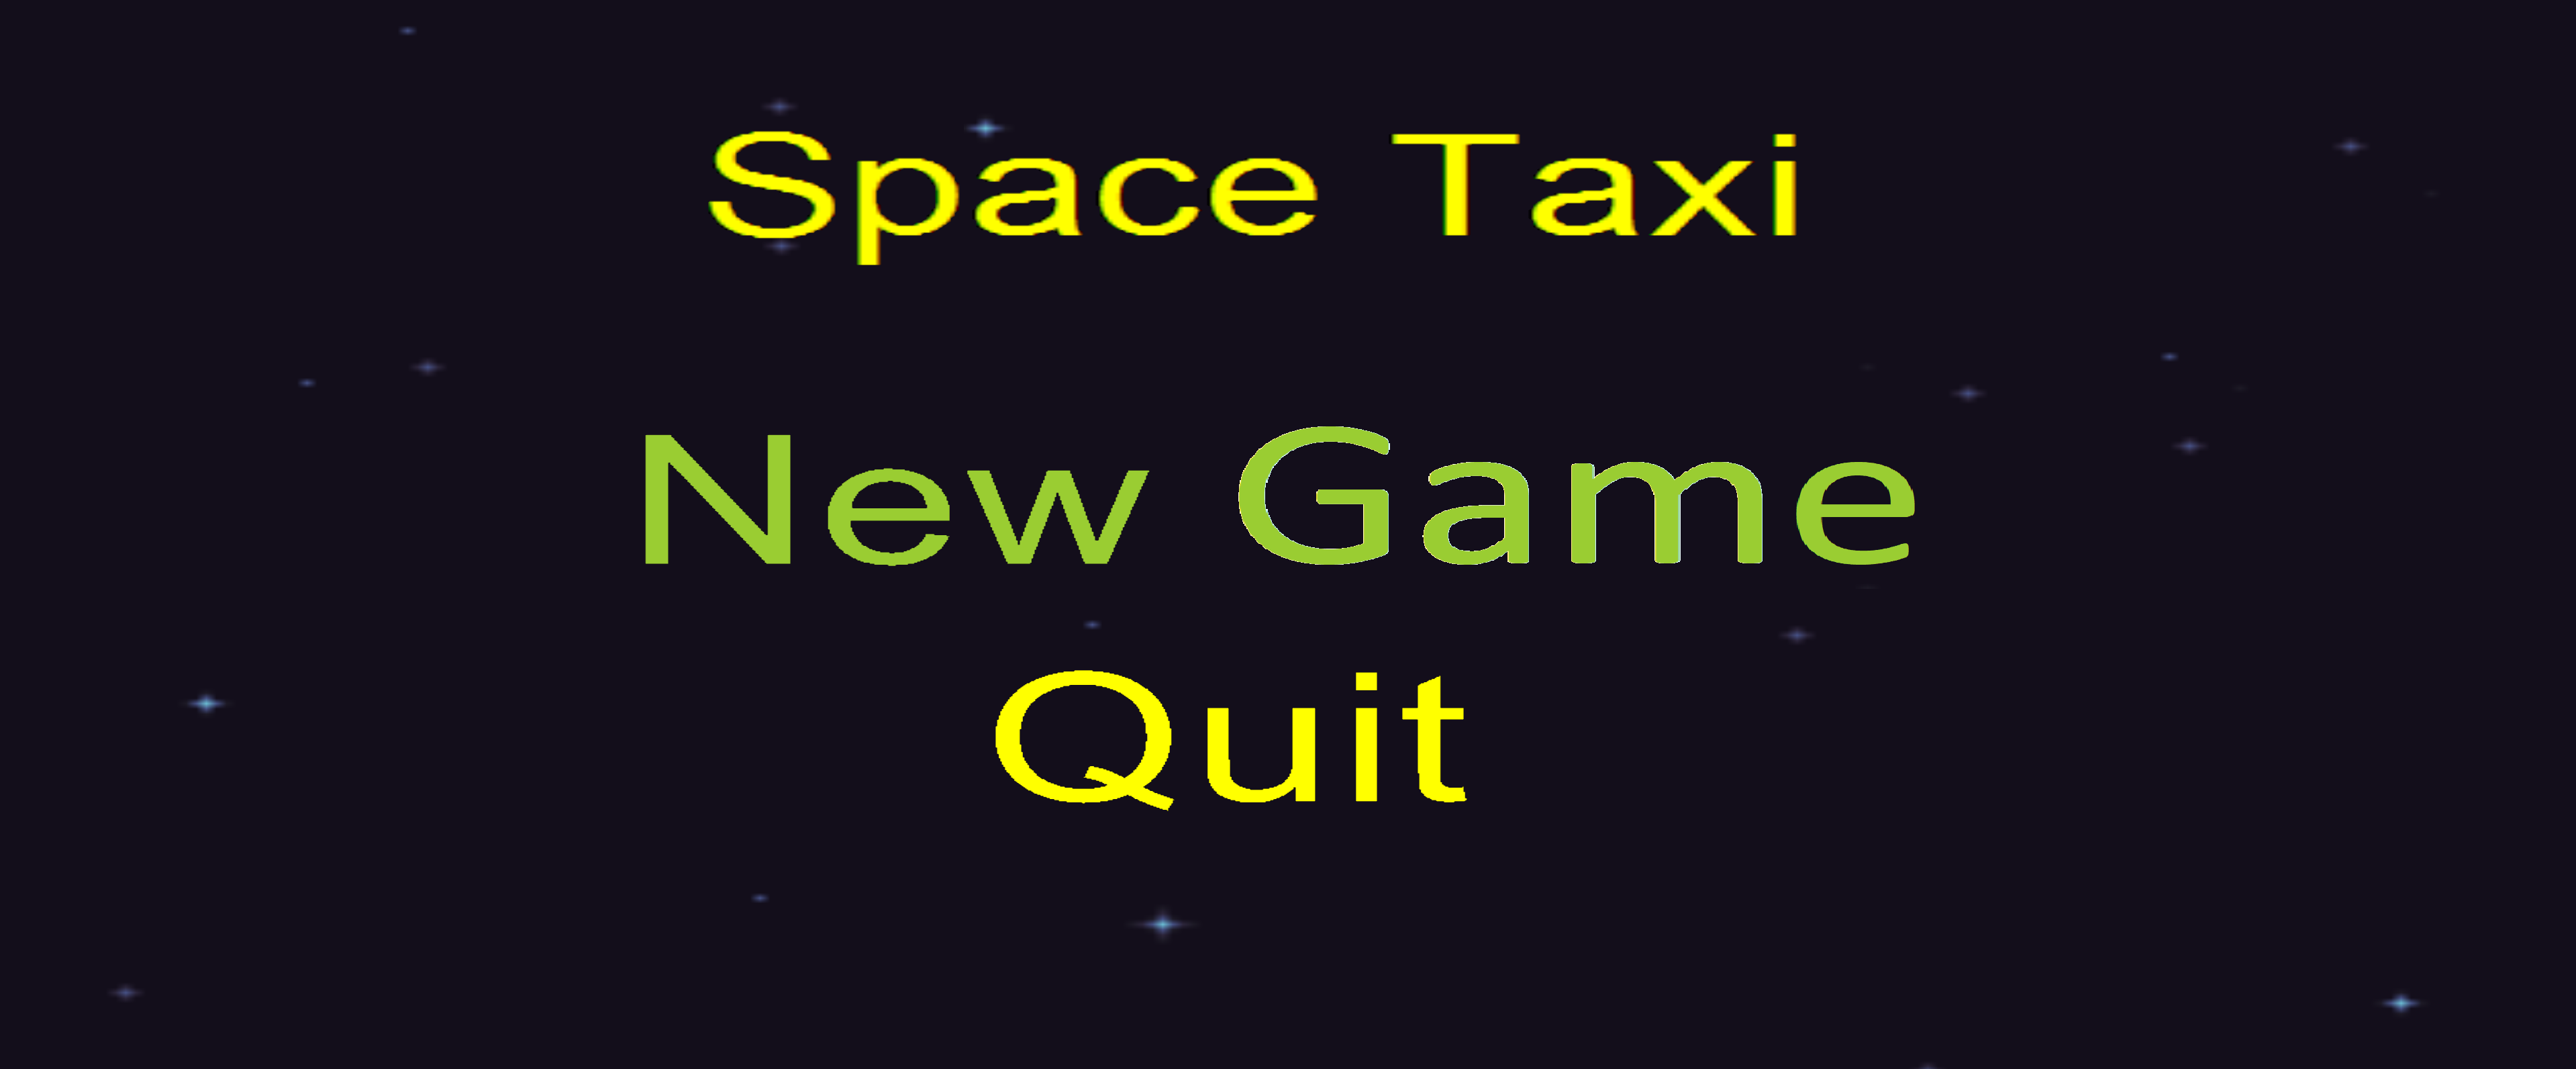
\includegraphics[width=1\textwidth]{./Pictures/MainMenu2.png}
\end{figure}

When starting the game, your job as a taxi driver in SPACE, is to get to your customer and pick them up at their platform where they are waiting. 
\begin{figure}[h]
	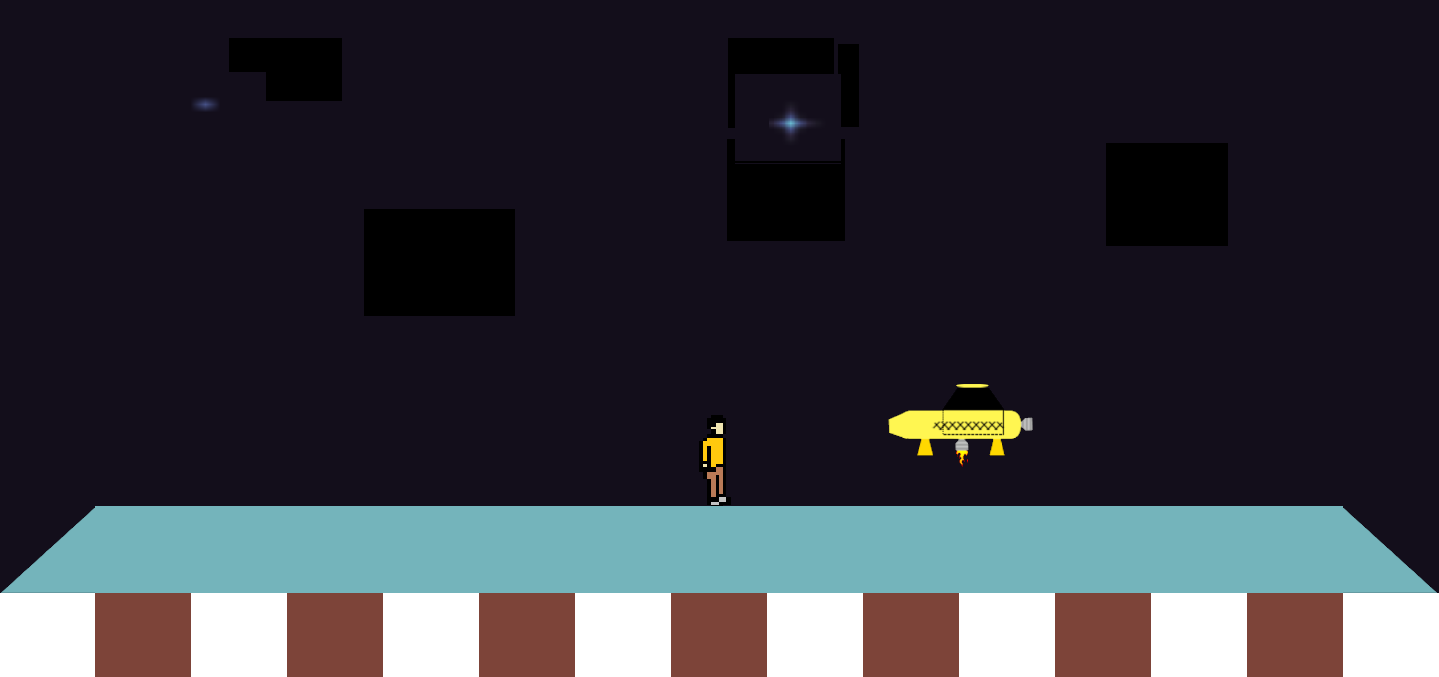
\includegraphics[width=1\textwidth]{./Pictures/SpaceTaxiLandingNew3.png}
\end{figure}

From here on, you should drop off your customers at their desired destination (next platform) in time or they might get angry at you and pay less money.\\

\newpage

To get to the next level when finished the current level, you should collide with the portal up in the top middle of the screen, that will teleport you to the next level.
\begin{figure}[h]
	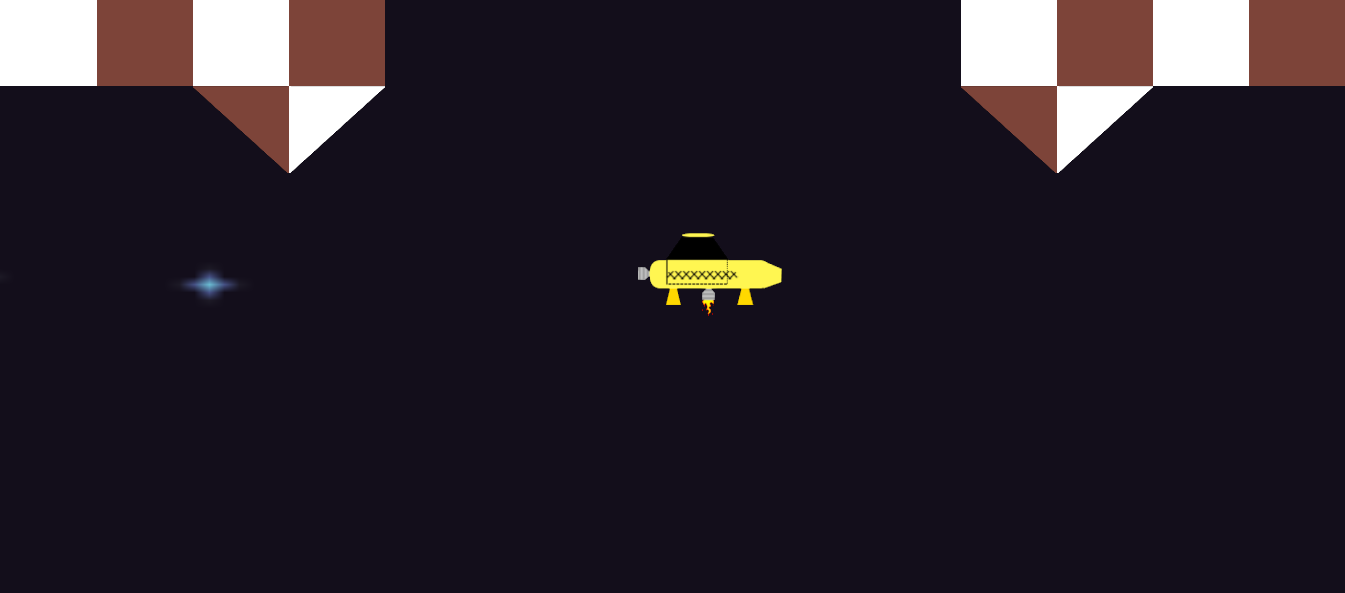
\includegraphics[width=1\textwidth]{./Pictures/SpaceTaxiPortal2.png}
\end{figure}

The next level will then be ``The Beach``:
\begin{figure}[h]
	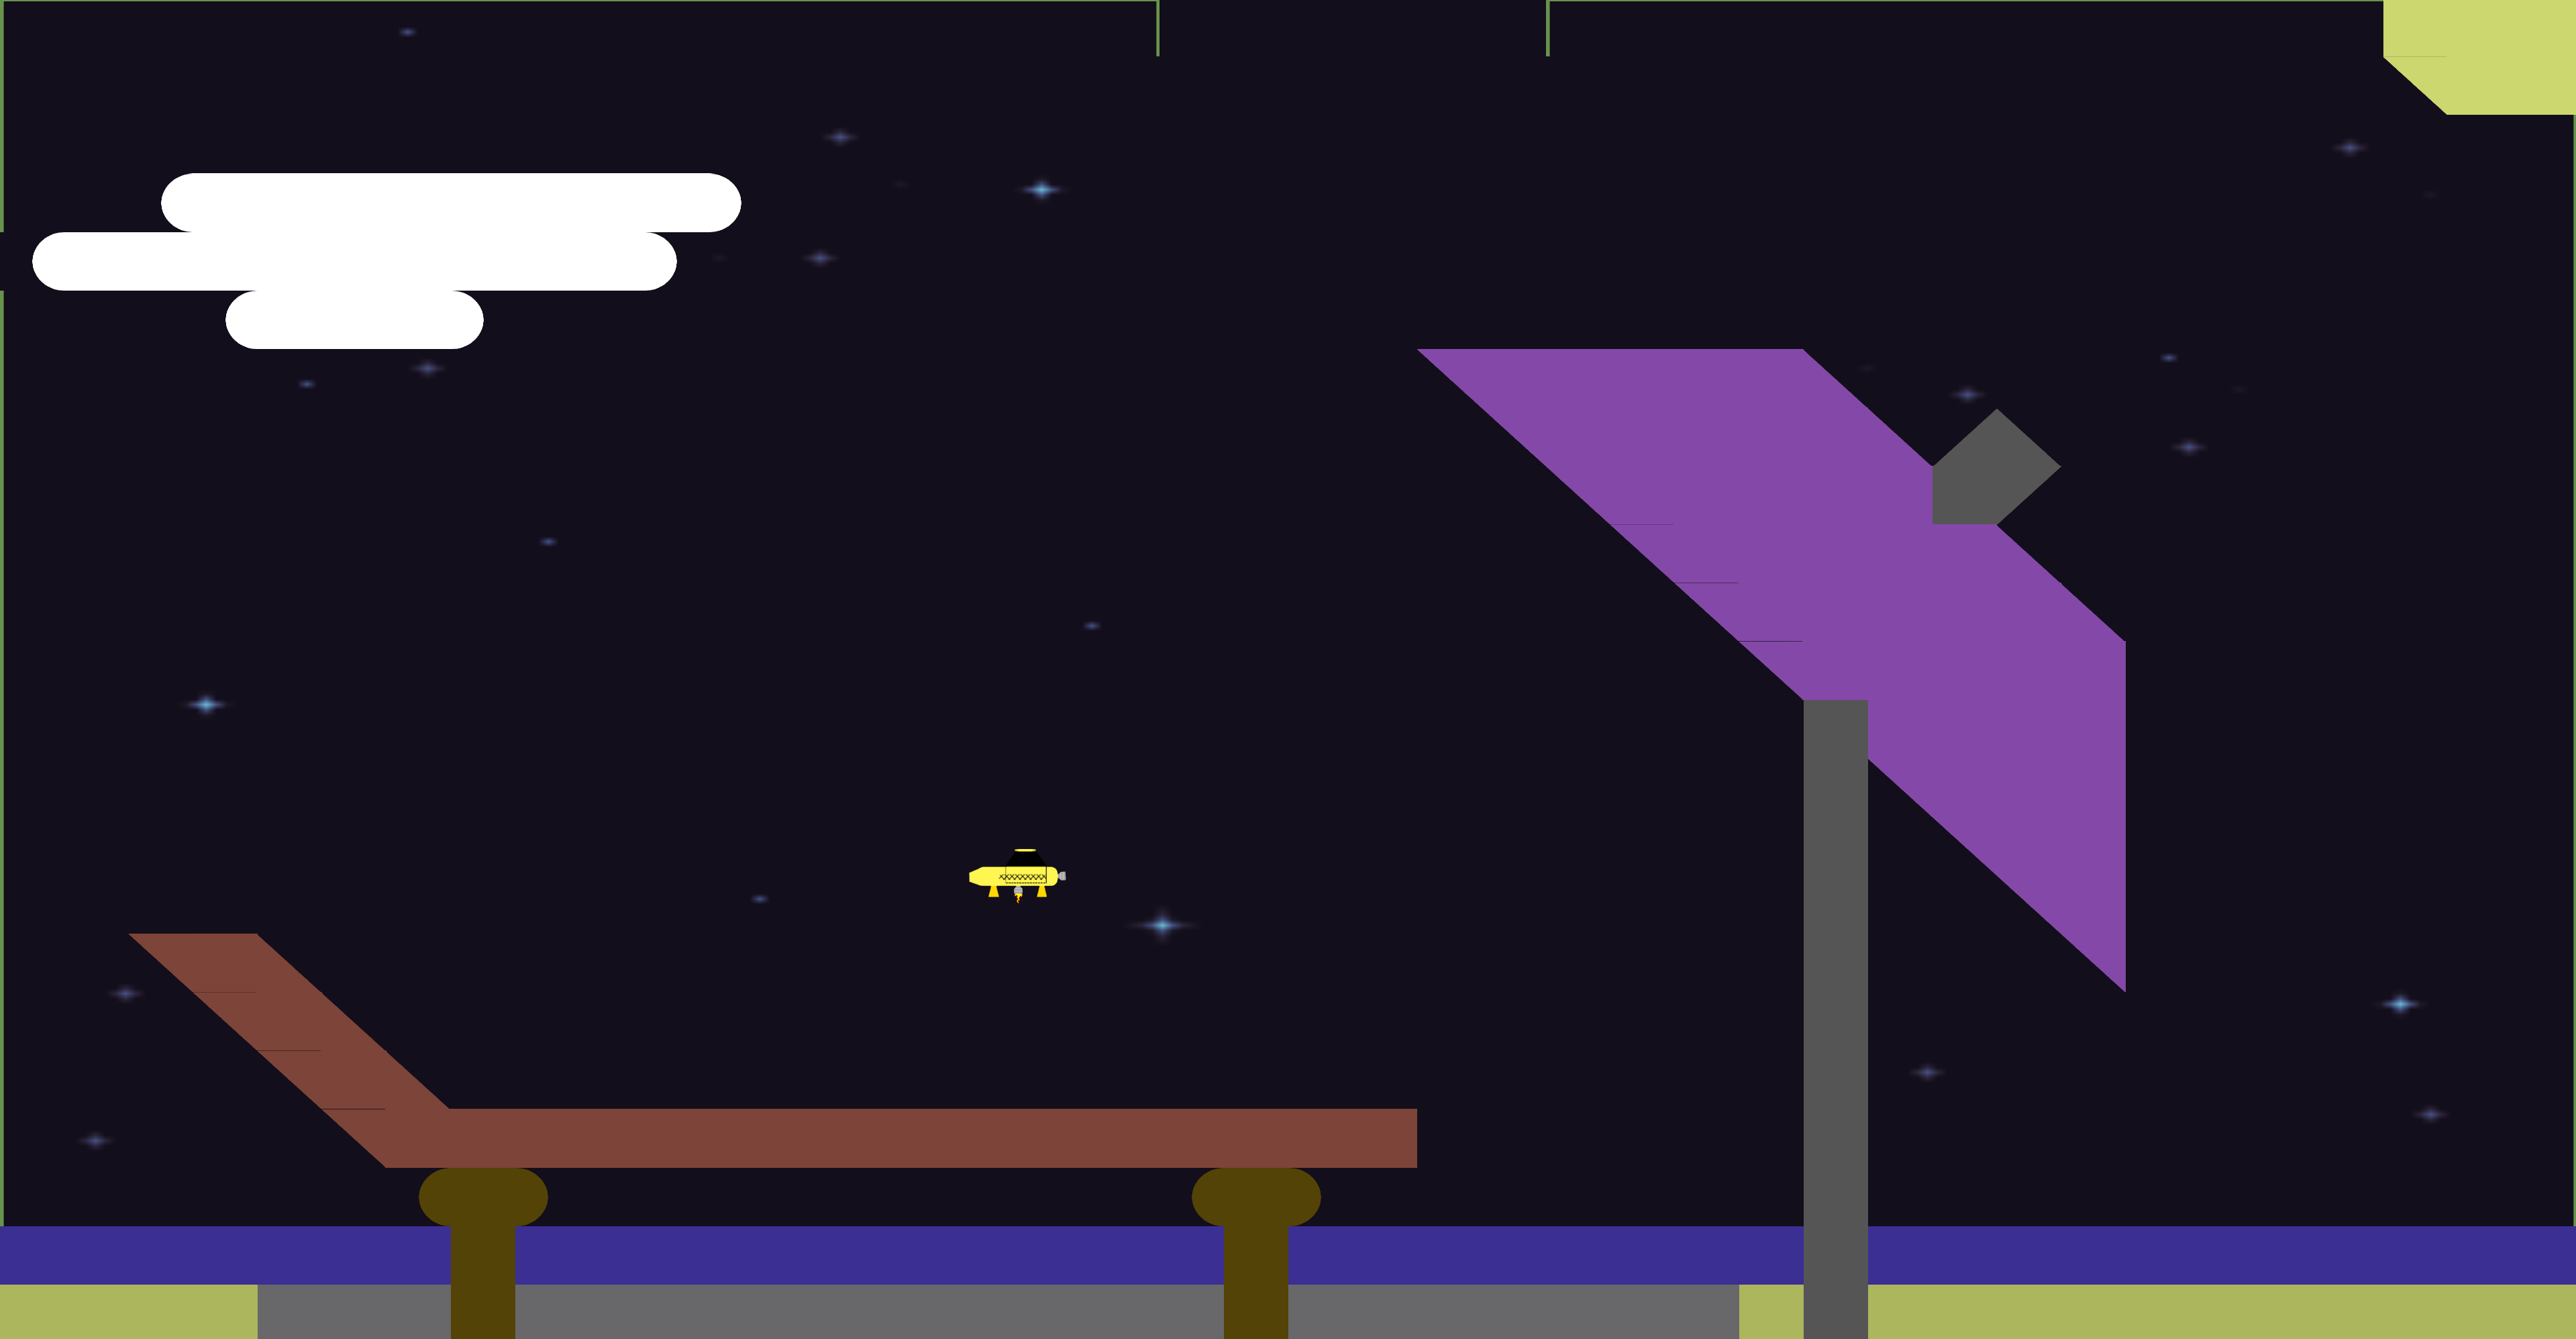
\includegraphics[width=1\textwidth]{./Pictures/TheBeach.png}
\end{figure}

\end{document}